\documentclass[12pt]{beamer}
\usetheme{Boadilla}
\usepackage{graphicx}
\usepackage{algorithm2e}
\graphicspath{{images/}}
\title{CMPT 155: Computer Applications for Life Sciences}
\subtitle{Lecture 4: Formatting Cells}
\author{Ivan E. Perez}
\institute{}
\date{January 26, 2022}
\usepackage{booktabs} % Allows the use of \toprule, 
\usepackage{appendix}
\usepackage{enumerate,multicol}
\usepackage{amsmath, amssymb, amsthm}
\usepackage{tikz}

\begin{document}
	\begin{frame}
		\titlepage
	\end{frame}
	\begin{frame}
		\frametitle{Presentation Outline}
		\tableofcontents
	\end{frame}
\section{Cell Formatting}
	\begin{frame}
		\frametitle{Formatting Cells}
			Cells formating options can be accessed through:
		\begin{itemize}
			\item Clicking home on the ribbon, $\rightarrow$ Cells $\rightarrow$ Format Cells
			\item Right-clicking (ctrl-click) on the cell and clicking \textit{Format Cell},
		\end{itemize} 
		\begin{center}
			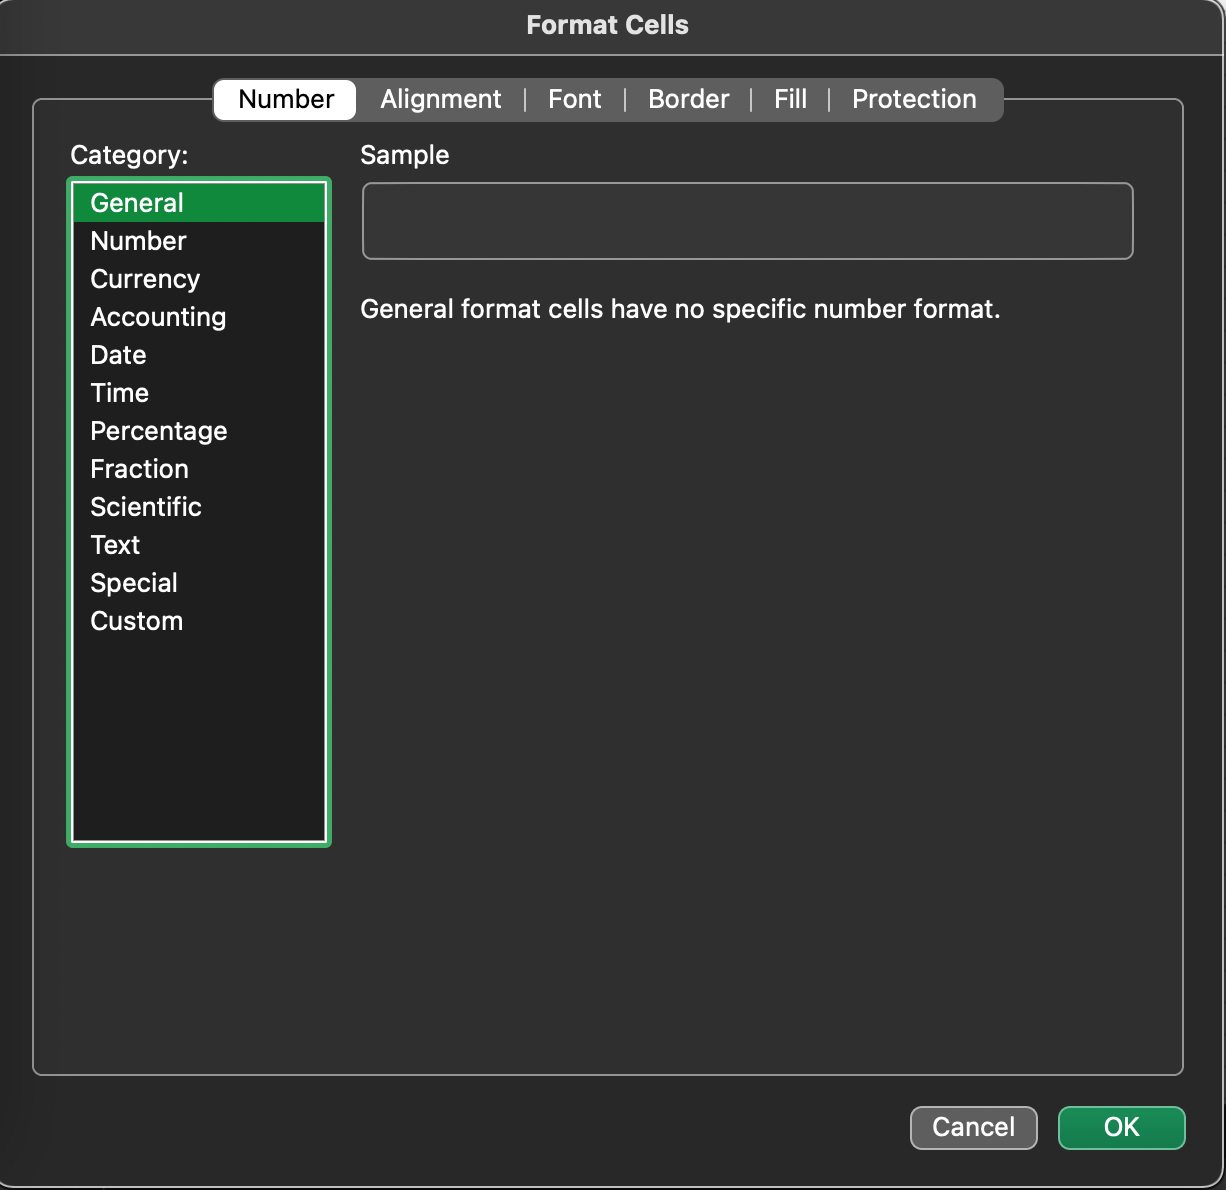
\includegraphics[width=0.5\textwidth]{formatcellsmenu.png}
		\end{center}
	\end{frame}
	\begin{frame}
	\frametitle{Various Cell Formats}
		\begin{center}
			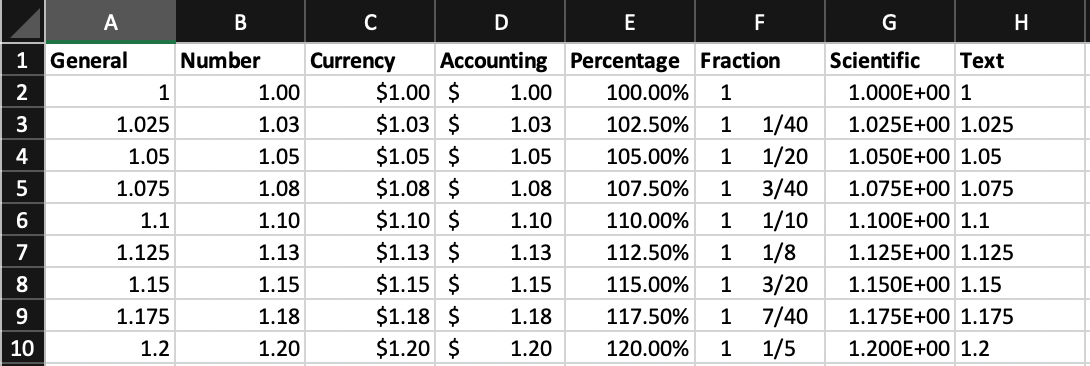
\includegraphics[width=\textwidth]{variouscellformats.png}
		\end{center}
	\end{frame}
	\begin{frame}
		\frametitle{Alignment and Orientation}
	\begin{itemize}
		\item Wrap Text
			\begin{itemize}
				\item Allows for a large amount of text to flow across multiple lines
				\item Click the wrap text icon in Home tab near the text alignment sections.
			\end{itemize}
		\item Mergeing Cells
			\begin{itemize}
				\item Home $\rightarrow$ Merge \& Center $\rightarrow$ Merge Cells.
				\item Make sure to have a whole selection of the cells you want to merge.
			\end{itemize}
		\item Rotating Content
			\begin{itemize}
				\item Rotate content by clicking the \textit{rotate content} icon near the text alignment sections.
			\end{itemize}
		\begin{center}
			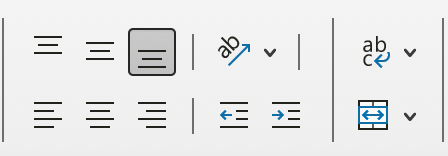
\includegraphics[width=0.4\textwidth]{wraprotatetext.png}
		\end{center}
	\end{itemize}
	\end{frame}

	\begin{frame}
		\frametitle{Fonts and Color}
		\begin{itemize}
			\item font style, size, style attributes (italics, underline bold), color
			\item special characters and emoji's! 
				\begin{itemize}
					\item  copyright symbol \textcopyright
					\item Insert $\rightarrow$ Symbols  $\rightarrow$ Symbol
				\end{itemize}
		\end{itemize}
		\begin{center}
			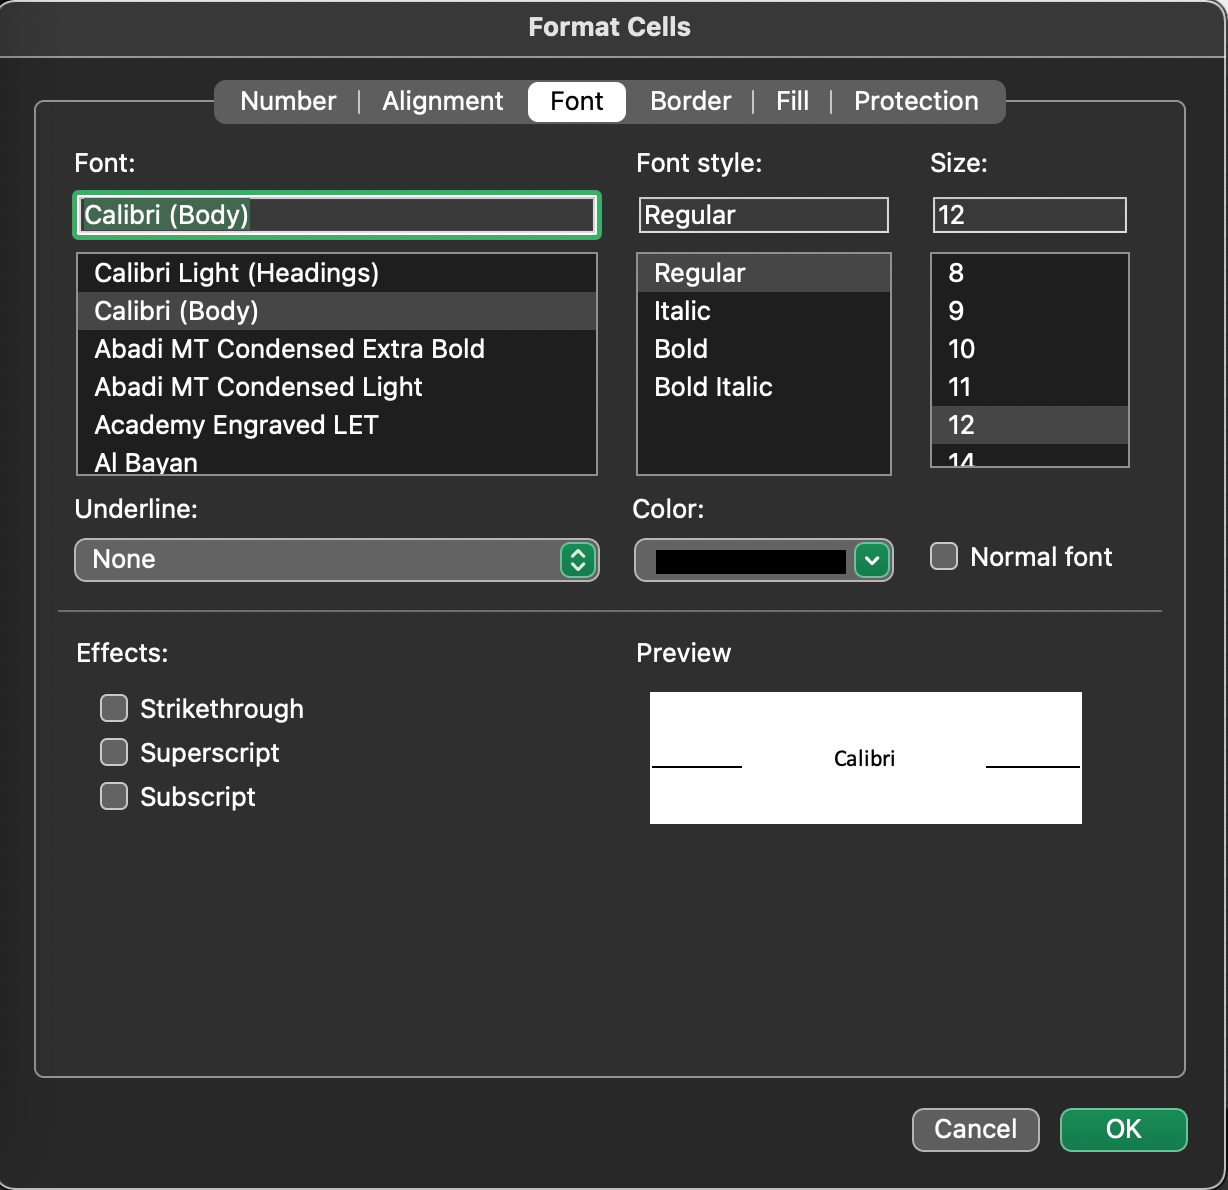
\includegraphics[width=0.5\textwidth]{cellformat_font_tab.png}
		\end{center}
	\end{frame}

	\begin{frame}
		\frametitle{Borders and Fills}
		\begin{itemize}
			\item Home$\rightarrow$Cells$\rightarrow$Format$\rightarrow$Format Cells \item right-click $\rightarrow$Format Cells $\rightarrow$ fill tab, border tab
		\end{itemize}
		\begin{figure}[htb]
			\begin{minipage}[t]{0.49\linewidth}\centering
				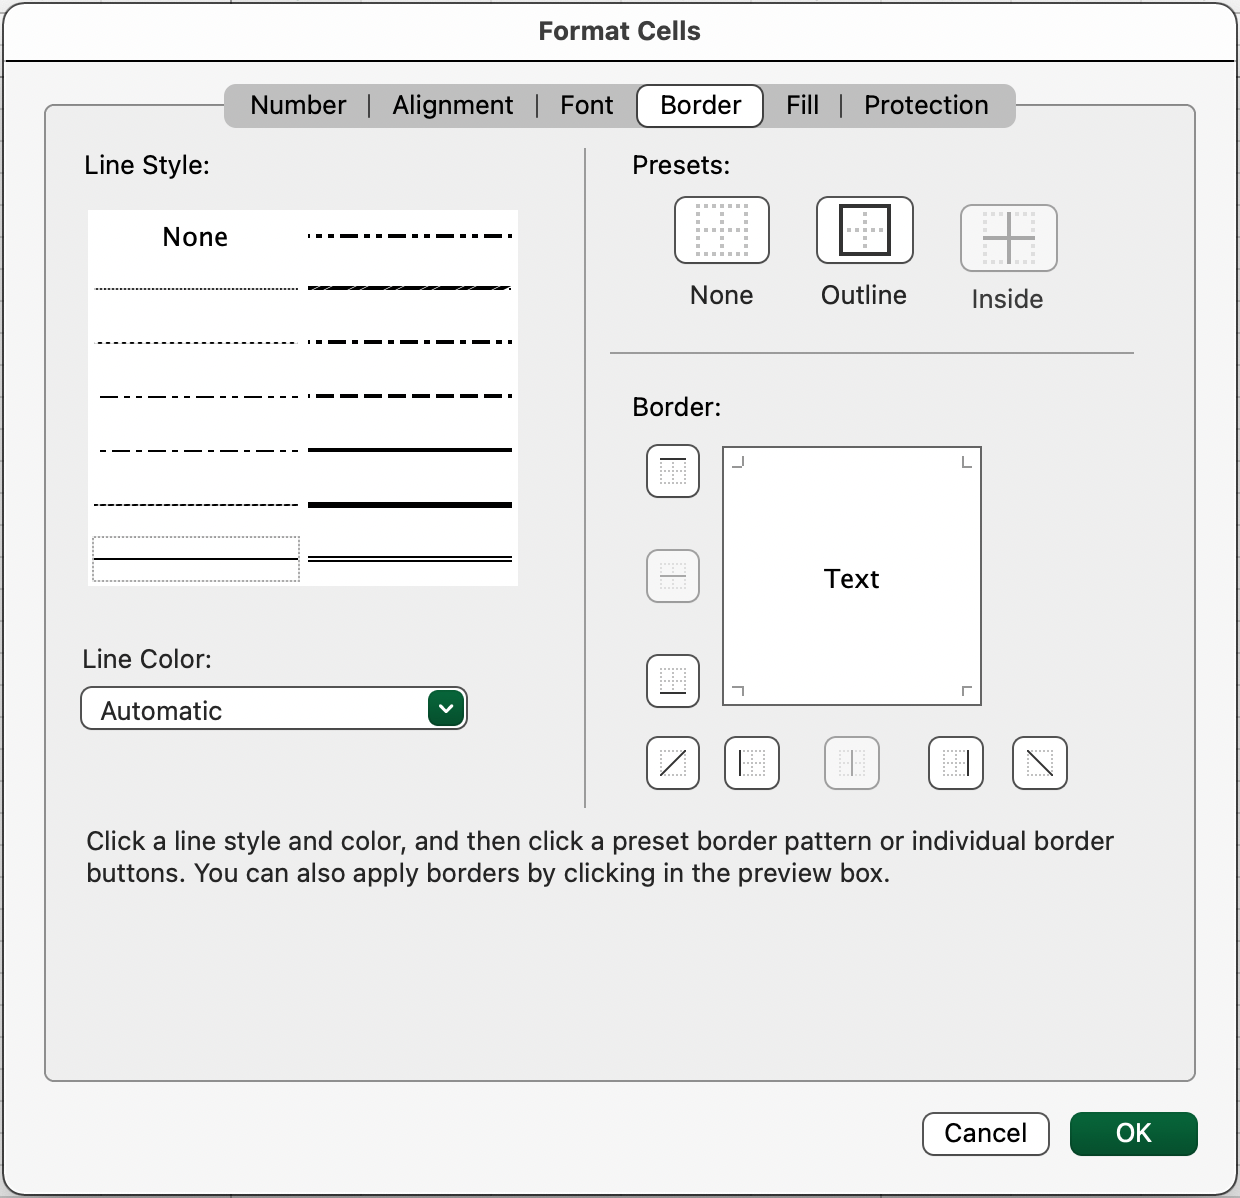
\includegraphics[width=0.75\linewidth]{cellformat_border_tab.png}
				\medskip
				\centerline{(a)}
			\end{minipage}\hfill
			\begin{minipage}[t]{0.5\linewidth}\centering
				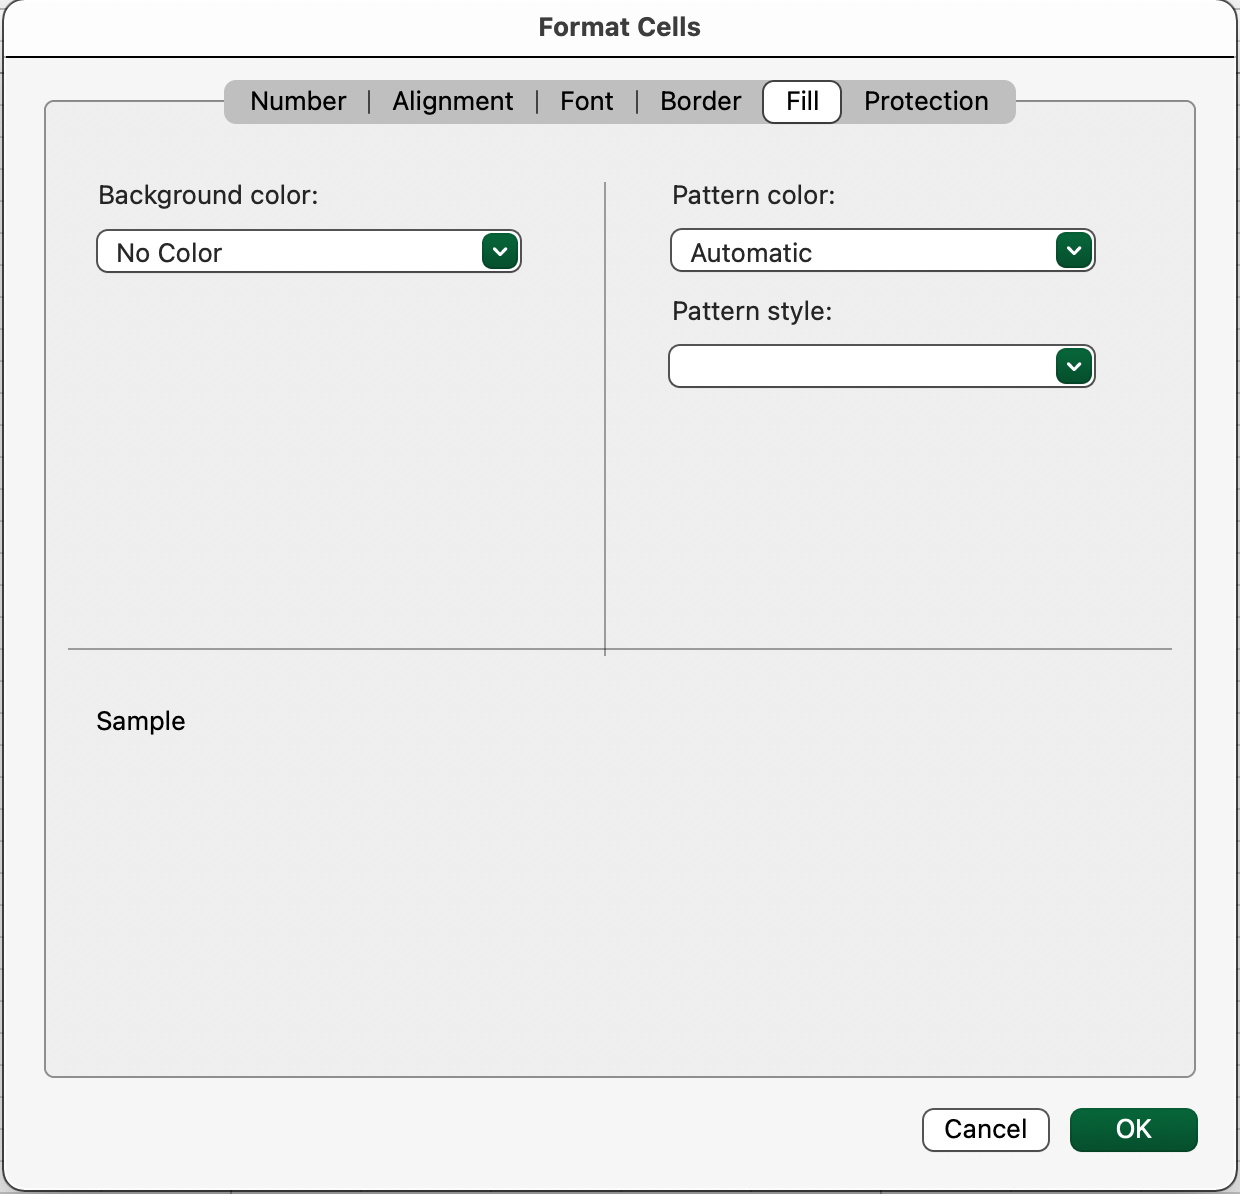
\includegraphics[width=0.75\linewidth]{cellformat_fill_tab.png}
				\medskip
				\centerline{(b)}
			\end{minipage}
			\caption{(a) shows the Border Tab, and (b) shows the Fill tab}
		\end{figure}
	\end{frame}

	\begin{frame}
		\frametitle{Highlting Specific Values}
		\begin{itemize}
			\item Conditional formatting rule
		 	\item A rule is an instruction that tells Excel when to apply conditional formatting to a cell and when to ignore it.
		 	\item Home $\rightarrow$ Styles $\rightarrow$ Conditional Formatting $\rightarrow$ Highlight Cells Rules
		\end{itemize}
		\begin{center}
			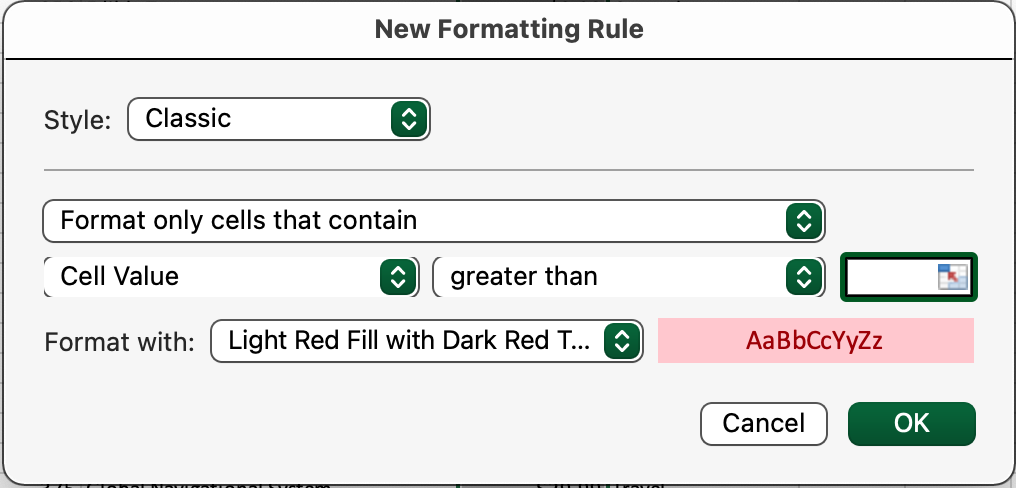
\includegraphics[width=0.5\textwidth]{conditionalformatting.png}
		\end{center}
		Lets try some formatting exercises by downloading \textit{Product.xlsx}
	\end{frame}
\section{Worksheet Visuals}
	\begin{frame}
		\frametitle{Zoom and Rearranging the Spread Sheet}
		\begin{itemize}
		 \item Zooming
		 \begin{itemize}
		 	 \item View $\rightarrow$ Zoom $\rightarrow$ Zoom
		 	 \item (bottom right side of screen) zoom percentage
		 	 \item (Office 365 web app) Ctrl(Cmd) + `+' , Ctrl(Cmd) + `-'
		\end{itemize}
		\item Viewing Distant Parts of a Spreadsheet at Once
		\item View$\rightarrow$Window$\rightarrow$Split
		\item \textit{demo}: What practical reasons are there view different parts of the spreadsheet/workbookv at once?
		\end{itemize}
	\end{frame}

	\begin{frame}
		\frametitle{Freezing Panes}
		\begin{itemize}
			\item to freeze the first column or first row
				\begin{itemize}
					\item View$\rightarrow$Window$\rightarrow$Freeze Panes$\rightarrow$Freeze Top Row
				\end{itemize}
			\item use Freeze Panes
			\begin{enumerate}
				\item place the cursor just-right of all the columns you want to freeze
				\item bring the cursor up(down) to just below all the rows you want to freeze
				\item go to `Freeze Panes'
				\item Freeze/Unfreeze Panes until you get a selection that works for you!
			\end{enumerate}
		\end{itemize}
	\begin{figure}	
		\begin{center}
			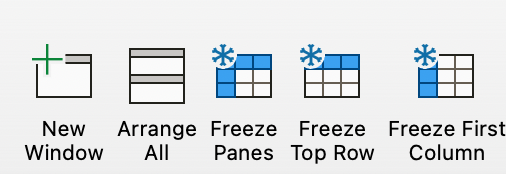
\includegraphics[width=0.4\textwidth]{freezepanes.png}
		\end{center}	
		\caption{freeze panes buttons in office 365}	
	\end{figure}
\end{frame}


\section{Printing and Page Layout}
	\begin{frame}
		\frametitle{Printing}
		 \begin{itemize}
		 	\item File $\rightarrow$Print or Ctrl (Cmd)
			\item Page Layout options 
			\begin{itemize}
				\item 
				\item Fit All Rows on One Page 
				\item Fit Sheet on One Page
			\end{itemize}
		\end{itemize}
	\begin{center}
		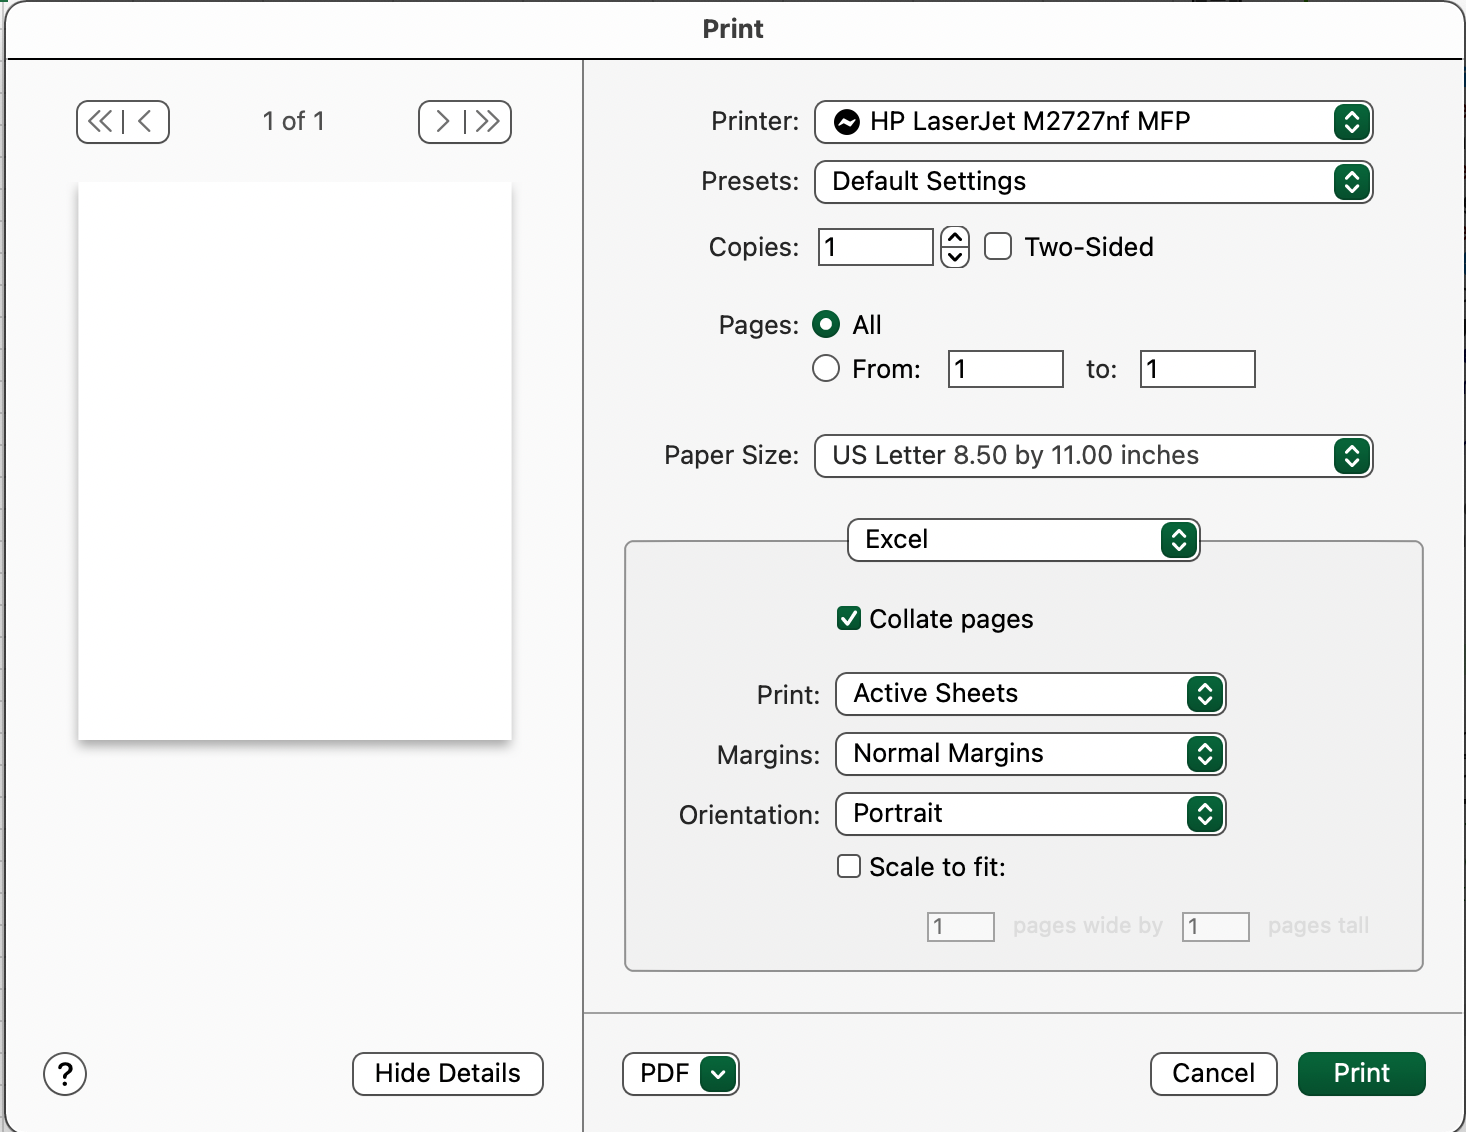
\includegraphics[width=0.5\textwidth]{printmenu.png}
	\end{center}
	\end{frame}
\end{document}

% things to do 
% pics replace, notes




